% Options for packages loaded elsewhere
\PassOptionsToPackage{unicode}{hyperref}
\PassOptionsToPackage{hyphens}{url}
%
\documentclass[
]{book}
\usepackage{amsmath,amssymb}
\usepackage{lmodern}
\usepackage{iftex}
\ifPDFTeX
  \usepackage[T1]{fontenc}
  \usepackage[utf8]{inputenc}
  \usepackage{textcomp} % provide euro and other symbols
\else % if luatex or xetex
  \usepackage{unicode-math}
  \defaultfontfeatures{Scale=MatchLowercase}
  \defaultfontfeatures[\rmfamily]{Ligatures=TeX,Scale=1}
\fi
% Use upquote if available, for straight quotes in verbatim environments
\IfFileExists{upquote.sty}{\usepackage{upquote}}{}
\IfFileExists{microtype.sty}{% use microtype if available
  \usepackage[]{microtype}
  \UseMicrotypeSet[protrusion]{basicmath} % disable protrusion for tt fonts
}{}
\makeatletter
\@ifundefined{KOMAClassName}{% if non-KOMA class
  \IfFileExists{parskip.sty}{%
    \usepackage{parskip}
  }{% else
    \setlength{\parindent}{0pt}
    \setlength{\parskip}{6pt plus 2pt minus 1pt}}
}{% if KOMA class
  \KOMAoptions{parskip=half}}
\makeatother
\usepackage{xcolor}
\usepackage{color}
\usepackage{fancyvrb}
\newcommand{\VerbBar}{|}
\newcommand{\VERB}{\Verb[commandchars=\\\{\}]}
\DefineVerbatimEnvironment{Highlighting}{Verbatim}{commandchars=\\\{\}}
% Add ',fontsize=\small' for more characters per line
\usepackage{framed}
\definecolor{shadecolor}{RGB}{248,248,248}
\newenvironment{Shaded}{\begin{snugshade}}{\end{snugshade}}
\newcommand{\AlertTok}[1]{\textcolor[rgb]{0.94,0.16,0.16}{#1}}
\newcommand{\AnnotationTok}[1]{\textcolor[rgb]{0.56,0.35,0.01}{\textbf{\textit{#1}}}}
\newcommand{\AttributeTok}[1]{\textcolor[rgb]{0.77,0.63,0.00}{#1}}
\newcommand{\BaseNTok}[1]{\textcolor[rgb]{0.00,0.00,0.81}{#1}}
\newcommand{\BuiltInTok}[1]{#1}
\newcommand{\CharTok}[1]{\textcolor[rgb]{0.31,0.60,0.02}{#1}}
\newcommand{\CommentTok}[1]{\textcolor[rgb]{0.56,0.35,0.01}{\textit{#1}}}
\newcommand{\CommentVarTok}[1]{\textcolor[rgb]{0.56,0.35,0.01}{\textbf{\textit{#1}}}}
\newcommand{\ConstantTok}[1]{\textcolor[rgb]{0.00,0.00,0.00}{#1}}
\newcommand{\ControlFlowTok}[1]{\textcolor[rgb]{0.13,0.29,0.53}{\textbf{#1}}}
\newcommand{\DataTypeTok}[1]{\textcolor[rgb]{0.13,0.29,0.53}{#1}}
\newcommand{\DecValTok}[1]{\textcolor[rgb]{0.00,0.00,0.81}{#1}}
\newcommand{\DocumentationTok}[1]{\textcolor[rgb]{0.56,0.35,0.01}{\textbf{\textit{#1}}}}
\newcommand{\ErrorTok}[1]{\textcolor[rgb]{0.64,0.00,0.00}{\textbf{#1}}}
\newcommand{\ExtensionTok}[1]{#1}
\newcommand{\FloatTok}[1]{\textcolor[rgb]{0.00,0.00,0.81}{#1}}
\newcommand{\FunctionTok}[1]{\textcolor[rgb]{0.00,0.00,0.00}{#1}}
\newcommand{\ImportTok}[1]{#1}
\newcommand{\InformationTok}[1]{\textcolor[rgb]{0.56,0.35,0.01}{\textbf{\textit{#1}}}}
\newcommand{\KeywordTok}[1]{\textcolor[rgb]{0.13,0.29,0.53}{\textbf{#1}}}
\newcommand{\NormalTok}[1]{#1}
\newcommand{\OperatorTok}[1]{\textcolor[rgb]{0.81,0.36,0.00}{\textbf{#1}}}
\newcommand{\OtherTok}[1]{\textcolor[rgb]{0.56,0.35,0.01}{#1}}
\newcommand{\PreprocessorTok}[1]{\textcolor[rgb]{0.56,0.35,0.01}{\textit{#1}}}
\newcommand{\RegionMarkerTok}[1]{#1}
\newcommand{\SpecialCharTok}[1]{\textcolor[rgb]{0.00,0.00,0.00}{#1}}
\newcommand{\SpecialStringTok}[1]{\textcolor[rgb]{0.31,0.60,0.02}{#1}}
\newcommand{\StringTok}[1]{\textcolor[rgb]{0.31,0.60,0.02}{#1}}
\newcommand{\VariableTok}[1]{\textcolor[rgb]{0.00,0.00,0.00}{#1}}
\newcommand{\VerbatimStringTok}[1]{\textcolor[rgb]{0.31,0.60,0.02}{#1}}
\newcommand{\WarningTok}[1]{\textcolor[rgb]{0.56,0.35,0.01}{\textbf{\textit{#1}}}}
\usepackage{longtable,booktabs,array}
\usepackage{calc} % for calculating minipage widths
% Correct order of tables after \paragraph or \subparagraph
\usepackage{etoolbox}
\makeatletter
\patchcmd\longtable{\par}{\if@noskipsec\mbox{}\fi\par}{}{}
\makeatother
% Allow footnotes in longtable head/foot
\IfFileExists{footnotehyper.sty}{\usepackage{footnotehyper}}{\usepackage{footnote}}
\makesavenoteenv{longtable}
\usepackage{graphicx}
\makeatletter
\def\maxwidth{\ifdim\Gin@nat@width>\linewidth\linewidth\else\Gin@nat@width\fi}
\def\maxheight{\ifdim\Gin@nat@height>\textheight\textheight\else\Gin@nat@height\fi}
\makeatother
% Scale images if necessary, so that they will not overflow the page
% margins by default, and it is still possible to overwrite the defaults
% using explicit options in \includegraphics[width, height, ...]{}
\setkeys{Gin}{width=\maxwidth,height=\maxheight,keepaspectratio}
% Set default figure placement to htbp
\makeatletter
\def\fps@figure{htbp}
\makeatother
\setlength{\emergencystretch}{3em} % prevent overfull lines
\providecommand{\tightlist}{%
  \setlength{\itemsep}{0pt}\setlength{\parskip}{0pt}}
\setcounter{secnumdepth}{5}
\usepackage{booktabs}
\ifLuaTeX
  \usepackage{selnolig}  % disable illegal ligatures
\fi
\usepackage[]{natbib}
\bibliographystyle{apalike}
\IfFileExists{bookmark.sty}{\usepackage{bookmark}}{\usepackage{hyperref}}
\IfFileExists{xurl.sty}{\usepackage{xurl}}{} % add URL line breaks if available
\urlstyle{same} % disable monospaced font for URLs
\hypersetup{
  pdftitle={Data Science for Social Scientists},
  pdfauthor={Daniel E. Ehrlich; Anna Tremblay},
  hidelinks,
  pdfcreator={LaTeX via pandoc}}

\title{Data Science for Social Scientists}
\author{Daniel E. Ehrlich \and Anna Tremblay}
\date{2022-08-16}

\begin{document}
\maketitle

{
\setcounter{tocdepth}{1}
\tableofcontents
}
\hypertarget{preface}{%
\chapter*{Preface}\label{preface}}
\addcontentsline{toc}{chapter}{Preface}

This is my very first bookdown book. I hope you like it.

\textbf{TIP:} Note the \texttt{\{-\}} used to indicate ``do not number this section'' eg: preface.

\hypertarget{course-structure}{%
\section{Course Structure}\label{course-structure}}

This syllabus is initially envisioned as 3 5-week sections. However, compilation and content are intended to be modular with templates for instructors to include their own specialties.

The basic structure of this course is:

\hypertarget{unit-1-understanding-and-testing-data}{%
\subsection{Unit 1 Understanding and Testing Data}\label{unit-1-understanding-and-testing-data}}

Students will be able to:

Technical:

\begin{itemize}
\tightlist
\item
  Download R and RStudio
\item
  Read data into R and
\item
  Write (save) data out of R.
\item
  Summarize data visually

  \begin{itemize}
  \tightlist
  \item
    Using base R
  \item
    Using ggplot (tidyverse)
  \end{itemize}
\item
  Summarize data tabularly

  \begin{itemize}
  \tightlist
  \item
    Using base R
  \item
    Using gttable / tidyverse
  \end{itemize}
\item
  Formally state and test assumptions of data

  \begin{itemize}
  \tightlist
  \item
    \emph{EG:} t-test, anova, (maybe) correlations
  \end{itemize}
\end{itemize}

Conceptual:

\begin{itemize}
\tightlist
\item
  Understand main types of data

  \begin{itemize}
  \tightlist
  \item
    \emph{EG:} logical, numeric, character, etc
  \item
    R specic vs general terms
  \end{itemize}
\item
  Recgonize various data distributions

  \begin{itemize}
  \tightlist
  \item
    \emph{EG:} normal, poisson, etc
  \end{itemize}
\item
  Know which types statistical tests are appropriate for a given set of data.
\end{itemize}

\hypertarget{unit-2-finding-data-and-asking-questions}{%
\subsection{Unit 2 Finding Data and Asking Questions}\label{unit-2-finding-data-and-asking-questions}}

Here we demonstrate two \textbf{different} approaches to conducting research.

\hypertarget{exploratory-analysis}{%
\subsubsection{Exploratory Analysis}\label{exploratory-analysis}}

If you've just collected a survey, or other raw data, you may not know what you're looking for. This is perfectly ok but goes against \emph{the scientific method} most people learned in grade school (More on that to follow(\textbf{\emph{include\_link}})).

This unit begins by presenting data/distributions and asking students to begin interpreting the data . visual exploration is encouraged and basic of data manipulation are taught
* \emph{EG:} how to subset data, how to reshape data, how to recode data, how to convert from one \texttt{data\ type} to another.

Example lab exercise:

Students given a data set (xls, csv, etc)
* load data, perform manipulations, basic summaries
+ cross tabs
+ group means by a covariate
* inspect data visually
+ \emph{DESCRIBE} the distribution - is it normal? significant?
* \emph{FIND} aquestion in the spread of the data
+ how can you test this (maybe small group work)
* write up/ present results
+ think on confounding factors / biases

\hypertarget{hypotethsis-driven}{%
\subsubsection{Hypotethsis Driven}\label{hypotethsis-driven}}

If, on the other hand you have an a pre-exisiting idea you want to test. We can follow the traditional \emph{scientific method}. With a question in mind, the first question is: where to look. What better place than \href{https://ipums.org}{IPUMS}!

Begin introducing navigation of web resources - mainly IPUMS international

Students should become comfortable working through lab exercises:
* Define a question (or be presented with one)
* Download variables from IPUMS (course downloads possible)
* Perform a basic analysis (discussed in Unit 1)
* Generate a \textbf{visual argument} for your analysis
+ Include explanation/interpretation/reflection on the question at hand, and the data used
+ Any obvious biases
+ Any obvious confounding factors

\hypertarget{unit-3-discussing-data-and-student-research}{%
\subsection{Unit 3 Discussing Data and Student Research}\label{unit-3-discussing-data-and-student-research}}

In this section we encourage the instructor to provide ample time for indepent student/small-group research. Some class time should be devoted to modelling healthy disussion and critique of methods.

We provide some examples here but encourage instrcutors (or students) to bring in recent journal/popular articles that do (or do not) apply data science methods well.

\hypertarget{guiding-principles}{%
\section{GUIDING PRINCIPLES}\label{guiding-principles}}

\begin{itemize}
\tightlist
\item
  phenomenon-based learning

  \begin{itemize}
  \tightlist
  \item
    try to start the class with a \textbf{question} or \textbf{problem}
  \item
    \emph{why} does the data look the way it does
  \item
    structure class so students work towards solving the problem
  \end{itemize}
\item
  RELEVANT examples

  \begin{itemize}
  \tightlist
  \item
    try to touch on 2 or more disciplines (eg, economics, demography)
  \end{itemize}
\end{itemize}

\hypertarget{dev-notes}{%
\section{DEV NOTES}\label{dev-notes}}

\hypertarget{to-do}{%
\subsection{TO DO}\label{to-do}}

\begin{itemize}
\tightlist
\item
  discuss style

  \begin{itemize}
  \tightlist
  \item
    key terms section for each chapter?
  \item
    key terms in \textbf{bold}
  \item
    italics for \emph{emphasis}
  \item
    are we pro-hyphens, or are they pedantic?
  \end{itemize}
\end{itemize}

\hypertarget{documentation}{%
\subsection{Documentation}\label{documentation}}

This function grabs any packages in your project and adds them to a local list that can be referenced using \texttt{R-pacakgename}
* \textbf{NOTE} in practice, that needs to be wrapped in markdown syntax, eg:
\texttt{{[}@R-bookdown{]}}
* See help files for more info - might be able to create/add a \texttt{citation} file

\hypertarget{intro}{%
\chapter{Introduction}\label{intro}}

Welcome to our open-source and cross-listed course on Data Science for kids who can't read data but want to learn to read data and other things too. in R.

We hope your knowledge of R increases, just like the graph below!
* (This is just making up reasons for the sample plot)

\begin{Shaded}
\begin{Highlighting}[]
\FunctionTok{par}\NormalTok{(}\AttributeTok{mar =} \FunctionTok{c}\NormalTok{(}\DecValTok{4}\NormalTok{, }\DecValTok{4}\NormalTok{, .}\DecValTok{1}\NormalTok{, .}\DecValTok{1}\NormalTok{))}
\FunctionTok{plot}\NormalTok{(pressure, }\AttributeTok{type =} \StringTok{\textquotesingle{}b\textquotesingle{}}\NormalTok{, }\AttributeTok{pch =} \DecValTok{19}\NormalTok{)}
\end{Highlighting}
\end{Shaded}

\begin{figure}

{\centering 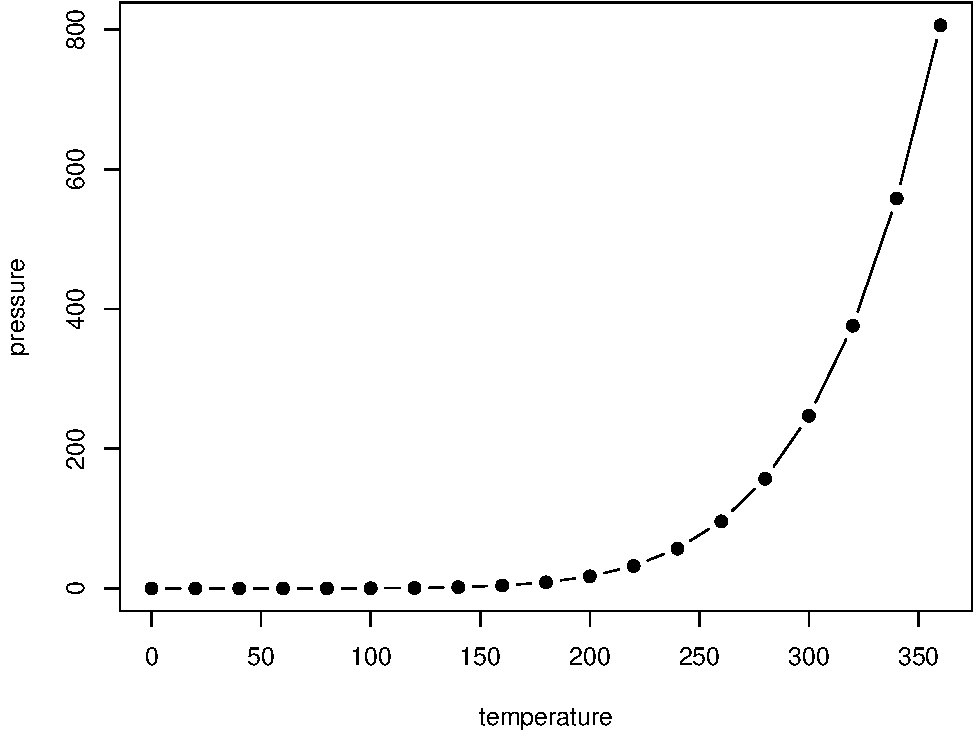
\includegraphics[width=0.8\linewidth]{_main_files/figure-latex/nice-fig-1} 

}

\caption{Here is a nice figure!}\label{fig:nice-fig}
\end{figure}

Reference a figure by its code chunk label with the \texttt{fig:} prefix, e.g., see Figure \ref{fig:nice-fig}. Similarly, you can reference tables generated from \texttt{knitr::kable()}, e.g., see Table \ref{tab:nice-tab}.

\begin{Shaded}
\begin{Highlighting}[]
\NormalTok{knitr}\SpecialCharTok{::}\FunctionTok{kable}\NormalTok{(}
  \FunctionTok{head}\NormalTok{(iris, }\DecValTok{20}\NormalTok{), }\AttributeTok{caption =} \StringTok{\textquotesingle{}Here is a nice table!\textquotesingle{}}\NormalTok{,}
  \AttributeTok{booktabs =} \ConstantTok{TRUE}
\NormalTok{)}
\end{Highlighting}
\end{Shaded}

\begin{table}

\caption{\label{tab:nice-tab}Here is a nice table!}
\centering
\begin{tabular}[t]{rrrrl}
\toprule
Sepal.Length & Sepal.Width & Petal.Length & Petal.Width & Species\\
\midrule
5.1 & 3.5 & 1.4 & 0.2 & setosa\\
4.9 & 3.0 & 1.4 & 0.2 & setosa\\
4.7 & 3.2 & 1.3 & 0.2 & setosa\\
4.6 & 3.1 & 1.5 & 0.2 & setosa\\
5.0 & 3.6 & 1.4 & 0.2 & setosa\\
\addlinespace
5.4 & 3.9 & 1.7 & 0.4 & setosa\\
4.6 & 3.4 & 1.4 & 0.3 & setosa\\
5.0 & 3.4 & 1.5 & 0.2 & setosa\\
4.4 & 2.9 & 1.4 & 0.2 & setosa\\
4.9 & 3.1 & 1.5 & 0.1 & setosa\\
\addlinespace
5.4 & 3.7 & 1.5 & 0.2 & setosa\\
4.8 & 3.4 & 1.6 & 0.2 & setosa\\
4.8 & 3.0 & 1.4 & 0.1 & setosa\\
4.3 & 3.0 & 1.1 & 0.1 & setosa\\
5.8 & 4.0 & 1.2 & 0.2 & setosa\\
\addlinespace
5.7 & 4.4 & 1.5 & 0.4 & setosa\\
5.4 & 3.9 & 1.3 & 0.4 & setosa\\
5.1 & 3.5 & 1.4 & 0.3 & setosa\\
5.7 & 3.8 & 1.7 & 0.3 & setosa\\
5.1 & 3.8 & 1.5 & 0.3 & setosa\\
\bottomrule
\end{tabular}
\end{table}

You can write citations, too. For example, we are using the \textbf{bookdown} package \citep{R-bookdown} in this sample book, which was built on top of R Markdown and \textbf{knitr} \citep{xie2015}.

Each \texttt{.Rmd} creates a unique \textbf{CHAPTER}.
* Organizing by content probably makes the most sense
* Gives more flexibility to adapt 2/3 class days.
* \emph{other thoughts??}

\hypertarget{unit1}{%
\chapter{The Basics}\label{unit1}}

For now, I have 3 main chapters for each of the main sections:
* Basics of data science / R \ref{unit1}
* Applications/critiques using IPUMS data \ref{unit2}
* Student-driven projects \ref{unit3}

Each of these \textbf{Chapters} contains multiple sections. We'll likely want to break these sections out into their own \texttt{.Rmd} files as they get fleshed out. For now, I'll try to keep the abundance of files limited.

\textbf{NOTE:} As these actually get filled out, we will probably want to insert different \texttt{part}s to the book (EG, the content of Unit 1 is covered in \texttt{Part\ I}).
* Declare parts with \texttt{\#\ (PART)\ Part\ I\ \{-\}} immediately before the first chapter \texttt{\#} it contains.

\hypertarget{intro-to-rrstudio}{%
\section{Intro to R/RStudio}\label{intro-to-rrstudio}}

\hypertarget{reading-data-distributions}{%
\section{Reading Data / Distributions}\label{reading-data-distributions}}

\hypertarget{what-is-a-normal-distribution}{%
\subsection{\texorpdfstring{What \emph{is} a \textbf{normal distribution}}{What is a normal distribution}}\label{what-is-a-normal-distribution}}

\hypertarget{how-normal-is-it}{%
\subsubsection{How normal is it?}\label{how-normal-is-it}}

show increasingly unclear examples of normal vs not

introduce tests of normality

\hypertarget{measuring-normality---single-sample}{%
\subsubsection{Measuring normality - single sample}\label{measuring-normality---single-sample}}

reinforce {[}concept of statistical{]} \textbf{normality}

is a value from a sample? - one way ttest
something about tails

\hypertarget{comparing-normality---two-saples}{%
\subsubsection{comparing normality - two saples}\label{comparing-normality---two-saples}}

standard / two-way t test

\hypertarget{comparing-more-than-two---anova}{%
\subsubsection{comparing more than two - ANOVA}\label{comparing-more-than-two---anova}}

\hypertarget{unit2}{%
\chapter{IPUMS}\label{unit2}}

Some text to break up the sub-section headers

\hypertarget{intro-to-ipums-website}{%
\section{Intro to IPUMS website}\label{intro-to-ipums-website}}

\hypertarget{background-on-ipums}{%
\subsection{background on ipums}\label{background-on-ipums}}

\hypertarget{navigating-website}{%
\subsection{navigating website}\label{navigating-website}}

Find certain (very common) variables to answer (common) social science questions.

We describe our methods in this chapter.

Math can be added in body using usual syntax as follows. This may be useful, particularly for explaining the math side of things.

\hypertarget{math-example}{%
\section{math example}\label{math-example}}

\(p\) is unknown but expected to be around 1/3. Standard error will be approximated

\[
SE = \sqrt(\frac{p(1-p)}{n}) \approx \sqrt{\frac{1/3 (1 - 1/3)} {300}} = 0.027
\]

You can also use math in footnotes like this\footnote{where we mention \(p = \frac{a}{b}\)}. Footnotes are helpful because they re-link to where you left off.

We will approximate standard error to 0.027\footnote{\(p\) is unknown but expected to be around 1/3. Standard error will be approximated

  \[
  SE = \sqrt(\frac{p(1-p)}{n}) \approx \sqrt{\frac{1/3 (1 - 1/3)} {300}} = 0.027
  \]}

The \texttt{longnote} footnote seems particularly useful.

\hypertarget{unit3}{%
\chapter{Independent Research}\label{unit3}}

By this point, students should be familiar with basic concepts from Chapter \ref{unit1}. These include:

\begin{itemize}
\tightlist
\item
  Basic Coding

  \begin{itemize}
  \tightlist
  \item
    read/write data in/out of R
  \item
    basic manipulations
  \end{itemize}
\item
  Theoretical Basis

  \begin{itemize}
  \tightlist
  \item
    looking at data distributions
  \item
    formal assessment of distributions
  \end{itemize}
\end{itemize}

Students will also be familiar with how these concepts are applied from Chapter \ref{unit2}. Hopefully students will be able to:

\begin{itemize}
\tightlist
\item
  Come up with a social science question they are interested in

  \begin{itemize}
  \tightlist
  \item
    Critically think about target variable(s) of interest. Any \emph{a priori} covariates? confounders?
  \item
    Acquire relevant data from IPUMS
  \item
    Analyze, Summarize, Visualize Data

    \begin{itemize}
    \tightlist
    \item
      scope and complexity at student/teach discretion
    \end{itemize}
  \item
    Present research to class

    \begin{itemize}
    \tightlist
    \item
      \textbf{potentially} critically discuss/evaluate each others work.
    \item
      \textbf{science is collaborative} everyone should be out to do their best work and represent the data as best we can. We all have conscious and unconscious biases, and the best way to confront them is share and receive (respectful) feedback.
    \end{itemize}
  \end{itemize}
\end{itemize}

During this Unit, we suggest giving ample class time for independent student research, peer-to-peer collaboration, and basic R/stats troubleshooting. This would also be a great time to model how to give respectful criticism by discussing recent research papers.
* We could maybe come up with 1-2 seed examples, with a few talking points

\hypertarget{example-one}{%
\section{Example one}\label{example-one}}

\hypertarget{example-two}{%
\section{Example two}\label{example-two}}

\hypertarget{ex_code}{%
\chapter{Example RMD code}\label{ex_code}}

For now, this chapter is a bit of a placeholder. I'm not sure what/how the \texttt{references.Rmd} file actually fits in to the code/construction (it looks automatic) so I want to keep that in place and need a section to note that.

I also want a more centralized reference point to put any example code I find helpful while working in R/bookdown. This section could get really unrully really fast, but oh well.

\hypertarget{core}{%
\section{Core}\label{core}}

\texttt{index.Rmd} is required and treated as file \texttt{00}. Chapters \emph{should} be numbered for ease of sorting but custom orders are possible by specifying filenames somewhere \textbf{in this file}

Remember each Rmd file contains one and only one chapter, and a chapter is defined by the first-level heading \texttt{\#}.
+ \textbf{IE} beyond the YAML header this file functions as a normal chapter since it starts with a top level header.
+ Note that \texttt{index.Rmd} has its own YMAL in addition to the various .yml files\ldots not sure exactly how these relate.

Reference a figure by its code chunk label with the \texttt{fig:} prefix, e.g., see Figure \ref{fig:nice-fig}. Similarly, you can reference tables generated from \texttt{knitr::kable()}, e.g., see Table \ref{tab:nice-tab}.
* Again, this prints an auto-generated numeral
* also leaving this in the context of the plots in Chapter \ref{intro}

You can write citations, too. See \texttt{knitr::write\_bib()} for more on this. Quick example from demo/index (may not work without write\_bib() though): we are using the \textbf{bookdown} package \citep{R-bookdown} in this sample book, which was built on top of R Markdown and \textbf{knitr} \citep{xie2015}.
* If included, ``Refernces'' section gets added to each chapter.
* Not exactly sure where

Embed html renders (EG, fancy tables (IPUMS\_var\_desc), or any shiny app) with \texttt{webshot} R package and \texttt{phantomJS}.

\begin{Shaded}
\begin{Highlighting}[]
\FunctionTok{install.packages}\NormalTok{(}\StringTok{"webshot"}\NormalTok{)}
\NormalTok{webshot}\SpecialCharTok{::}\FunctionTok{install\_phantomjs}\NormalTok{()}
\end{Highlighting}
\end{Shaded}

\hypertarget{tips}{%
\section{Tips}\label{tips}}

\textbf{LABEL EVERYTHING} you'll likely want to reference it later
* code chunks that produce figures can be referenced via \texttt{@\textbackslash{}ref(fig:{[}LABEL{]})}

You can label chapter and section titles using \texttt{\{\#label\}} after them, e.g., we can reference Chapter \ref{intro}. If you do not manually label them, there will be automatic labels anyway, e.g., Chapter \ref{unit1}.
* No idea how the automatic references work, so always be sure to declare them.
* \textbf{NOTE} these display as the relevant Chapter \texttt{numeral}.

\hypertarget{syntax}{%
\section{Syntax}\label{syntax}}

\emph{italics} or
\emph{italics} (can handle spaces)
\textbf{bold}
\texttt{code}
\(equations\)

\hypertarget{math}{%
\subsection{Math}\label{math}}

Randal Pruim features an extensive list of common math expression on their \href{https://rpruim.github.io/s341/S19/from-class/MathinRmd.html}{github page}. Here are some quick notes:

In-line equations can be written within \texttt{\$} and will be displayed right there: \(a^2 + b^2 = c^2\). In contrast, you can also add equation chunks by using \texttt{\$\$}

This can be coded in-line, \[\sum_{n=1}^{10} n^2\], but will result in a page break.

Alternatively, a more ``classic'' equation chunk:

\$\$
Plain text doesnt get spaces

how

very

odd

\$\$

To compile this example to PDF, you need XeLaTeX. You are recommended to install TinyTeX (which includes XeLaTeX): \url{https://yihui.name/tinytex/}.

  \bibliography{book.bib,packages.bib}

\end{document}
